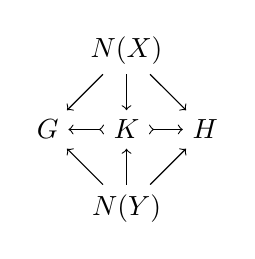
\begin{tikzpicture}
\node (v1) at (0,0) {$G$};
\node (v2) at (1,1) {$N(X)$};
\node (v3) at (1,0) {$K$};
\node (v4) at (1,-1) {$N(Y)$};
\node (v5) at (2,0) {$H$};
\draw [>->]  (v3) edge (v1);
\draw [>->] (v3) edge (v5);
\draw [->] (v2) edge (v1);
\draw [->] (v4) edge (v1);
\draw [->] (v2) edge (v3);
\draw [->] (v4) edge (v3);
\draw [->] (v2) edge (v5);
\draw [->] (v4) edge (v5);
\end{tikzpicture}